\documentclass{beamer}
\usetheme[color=ACMblue]{ACMNew}
\usepackage{beamernotes}
\usepackage{algpseudocodex}
\usepackage{listings}
\usepackage{lipsum}
\usetikzlibrary {automata,positioning,calc,shapes.geometric} 
\pdfcompresslevel=9
\pdfobjcompresslevel=3

\title[ACM fun]{CS 374A Midterm 1 Review}
\author{ACM @ UIUC}
%\institute{The Mental Institute}
\date{September 28, 2024}

\begin{document}

\begin{frame}
  \titlepage
\end{frame}
\bnote{This generates notes for pdfpc. These notes also appear
  on the handout/article versions.}

\begin{frame}[t]{Disclaimers and Logistics}
  \begin{itemize}
  \item \alert{Disclaimer:} Some of us are CAs, but we have not seen the exam. We have no idea what the questions are. However, we've taken the course and reviewed Sariel's previous exams, so we have \alert{suspicions} as to what the questions will be like.
  \item This review session is being recorded. Recordings and slides will be distributed on EdStem after the end.
  \item \alert{Agenda:} We'll quickly review all topics likely to be covered, then go through a practice exam, then review individual topics by request.
  \begin{itemize}
      \item Questions are designed to be written in the same style as Sariel's previous exams but to be \textit{slightly} harder, so don't worry if you don't get everything right away!
  \end{itemize}
  \item Please let us know if we're going too fast/slow, not speaking loud enough/speaking too loud, etc.
  \item If you have a question anytime during the review session, please ask! Someone else almost surely has a similar question.
  \item We'll provide a feedback form at the end of the session.
  \end{itemize}
\end{frame}

\begin{frame}[t]{Induction}
    \begin{exampleblock}{Template}
    Let $x$ be an \textit{arbitrary} <OBJECT>. Assume for all $k$ s.t. $k$ is smaller than $x$ (by <ORDERING PROPERTY>), that $P(k)$ holds.

    \vspace{.5cm}
    
    If $x =$ <MINIMAL OBJECT>, then $\dotsc$, so $P(x)$ holds

    \vspace{.5cm}

    If $x \neq$ <MINIMAL OBJECT>, then $\dotsc$, so by IH, $\dotsc$, so $P(x)$ holds.

    \vspace{.5cm}

    Thus, in all cases, $P(x)$ holds.
    \end{exampleblock}
    \vspace{.7 cm}
    \pause Some tips:
    \begin{itemize}
        \item \alert{Always use strong induction}. All weak inductive proofs can be re-written to use strong induction with minimal changes, and the extra assumption can make your life significantly easier.
        \item \alert{Write out your IH, base case, and inductive step out explicitly.} Doing so will help you avoid getting confused, and will help you avoid losing points.
        \item If you're performing induction on a recursive definition (strings, CFLs, etc.), generally, your inductive step will consist of one step of the recursion, and then will use IH.
    \end{itemize}
\end{frame}

\begin{frame}[t]{Regular Languages/Expressions}
    \begin{itemize}
        \item Built inductively on 3 operations:
        \begin{itemize}
            \item \pause $+$ is the union operator. $L(r_1 + r_2) = L(r_1) \cup L(r_2)$
            \item \pause $*$ is the Kleene star. $L(r_1^*) = L(r_1)^*$
            \item \pause $()$ are used to group expressions
            \item \pause (implicit) concatenation operator: $L(r_1r_2) = \{xy : x \in L_1, y \in L_2\}$
        \end{itemize}
        \item \pause Closed under Union ($\cup$), intersection ($\cap$), concatenation ($\cdot$), kleene star (${}^*$), complement ($^C$), set difference ($\setminus$), and reverse (${}^R$)
        \begin{itemize}
            \item \pause ... but only finitely many applications of these operations
        \end{itemize}
        \item \pause If trying to guess whether or not a language is regular, think about memory. When processing a string through a DFA, you only need to know which state you're currently in, and do not need to look forwards/backwards in the string.
        \begin{itemize}
            \item Implementing a DFA/NFA in code only requires $O(1)$ memory
            \item If your checker program needs to count something without bound, the language you're checking isn't regular.
        \end{itemize}
        \item \pause \alert{Regex Design Tips:} If you don't know where to start, try giving examples for strings that are in the language and strings that aren't. Look for patterns and try to build components around those patterns, then combine into something that represents the full language. Make sure to test and modify for edge cases. Explain, in English, each part of your regular expression with a short sentence. Does the explanation match the language?
    \end{itemize}
\end{frame}

\begin{frame}[t]{DFAs/NFAs}
    \begin{itemize}
        \item DFAs defined by \textit{state set} $Q$, \textit{accepting set} $A \subseteq Q$, \textit{input alphabet} $\Sigma$, \textit{start state} $s \in Q$, and \textit{transition function} $\delta: Q \times\Sigma \rightarrow Q$
        \item NFAs allow for ``trying'' multiple transitions at the same time or transitioning without reading in ($\epsilon$-transitions), accepts if there is a path to an accepting state. Transition function thereby changes to $\delta: Q \times(\Sigma \cup\{\epsilon\}) \rightarrow 2^Q$
        \begin{itemize}
            \item Power-set construction to convert from NFA to DFA- in theory exponential-time but used in practice.
        \end{itemize}
        \item \alert{Tips for creating DFA/NFAs}: Break down your language into smaller patterns, and figure out what you need to store as state for each part. Make sure you clearly define all components. A drawing or transition table is just as valid as a $(Q,A,\Sigma, s, \delta)$ definition. \pause
        \begin{block}{Product Constructions}
            Given some languages $L_1, \dots, L_n$ we want a DFA that accepts strings $w$ satisfying $f(w \in L_1,\dots,w \in L_n)$ where $f$ is some logical function. Create a DFA/NFA for $L$ using the following \textit{rough} format:
            \begin{itemize}
                \item $Q = Q_1 \times \cdots \times Q_n$
                \item $\delta'(q_1,\dots,q_n) = (\delta_1(q_1),\dots,\delta_2(q_2))$
                \item $s = (s_1,\dots,s_n)$
                \item $A' = \{\text{convert $f$ into a set expression}\}$
            \end{itemize}
        \end{block}
    \end{itemize}
\end{frame}

\begin{frame}[t]{Fooling Sets}
    \begin{itemize}
        \item DFAs only care about which state you're in, and not how you got there
        \begin{itemize}
            \item If two strings result in the same DFA state, any additional suffix added to both will also result in both strings being in the same state.
            \item \pause Thus, if we have $w, w'$, and we know that there exists a \alert{distinguishing suffix} $z$ s.t. $wz \in L, w'z \not\in L$, then $w, w'$ must be in \textit{different} states for \textit{any} DFA that accepts $L$ 
        \end{itemize}
        \item\pause A \alert{fooling set} is a set of strings where there exists a distinguishing suffix between every pair of strings
        \item Myhill-Nerode: min DFA size = max fooling set size
        \begin{itemize}
            \item \pause Thus, languages with infinite fooling sets are \textit{not} regular
        \end{itemize}
        \item \pause If you see the need to keep track of something without bound, you can create a fooling set around the part where you count up.
        \item \pause \alert{If you see divisibility, think primes!} All primes are coprime, so primality provides for an infinite set with easier construction of distinguishing suffixes.
        \item \pause If you're using strings of the form $1^k, 0^p$, etc. when sampling elements of your fooling set $a^i, a^j$, it's completely fine to assume WLOG that $j > i$, but nothing about the underlying structure of $i$ and $j$. If you want to put in such a restriction, you should instead restrict your fooling set further.
    \end{itemize}
\end{frame}

\begin{frame}[t]{Language Transforms}
    \begin{itemize}
        \item Used to prove that regularity is closed under some function $f$ (if $L$ is regular, then $f(L)$ is regular).
        \item \alert{General Format:} Given a DFA $M$ that accepts $L$, create an NFA $M'$ that accepts $f(L)$.
        \item \pause \alert{General Strategy:} Apply non-determinism to guess the future behavior of the DFA that you want to simulate.\pause
        \vspace{1 cm}
        \begin{alertblock}{Make sure you're going in the right direction!}
            If you see the format $f(L) = \{k(w) : w \in L\}$, your modified NFA should be trying to \textit{undo} $k$, while if you see the format $f(L) = \{w : k(w) \in L\}$, your modified NFA should be trying to \textit{apply} $k$. Mixing these up is the most common mistake we see on homeworks/exams.

            \vspace{.25cm}
            
            In some cases, only one direction is possible. For example, $\texttt{un-palin}(L): \{w : ww^R \in L\}$ has a transformation construction, but $\texttt{palin}(L) = \{ww^R: w \in L\}$ is irregular for some $L$.
        \end{alertblock}
    \end{itemize}
\end{frame}

\begin{frame}[t]{Context-Free Languages/Grammars}
    \begin{itemize}
        \item Formally, a context-free grammar is defined by \textit{nonterminals/variables} $V$, \textit{terminals/symbols} $T$, \textit{productions} $P$, 
        and the \textit{start symbol} $S$. Each production rule in $P$ looks like $A \to \alpha$, where $A \in V$ and $\alpha \in (V \cup T)^*$.

        \item \pause For example, consider $V = \{S\}, T=\{0,1\}, P=\{S \to \epsilon, S \to 0S1 \}$. (You can abbreviate this to $P=\{S \to \epsilon \mid 0S1 \}$.) What language is this?

        \begin{exampleblock}{Intuition}
            CFGs "build" strings, going from the outside in; you can choose rules to add characters on the left/right.
            
            Alternatively, CFGs "peel back" strings, removing characters from the left/right until nothing is left.
        \end{exampleblock}

        \item \pause CFLs only closed under union, kleene star, and concatenation. CFLs are \textit{not} closed under intersection or complement.

    \end{itemize}

    \pause \begin{center}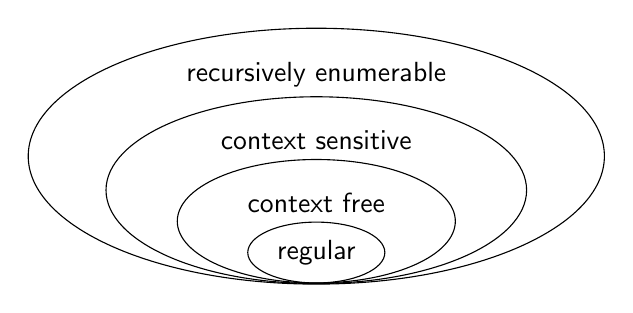
\begin{tikzpicture}[font=\sffamily,breathe dist/.initial=2ex]
    \foreach \X [count=\Y,remember=\Y as \LastY] in 
    {regular,context free,context sensitive,recursively enumerable}
     {\ifnum\Y=1
      \node[ellipse,draw,outer sep=0pt] (F-\Y) {\X};
     \else
      \node[anchor=south] (T-\Y) at (F-\LastY.north) {\X};
      \path let \p1=($([yshift=\pgfkeysvalueof{/tikz/breathe dist}]T-\Y.north)-(F-\LastY.south)$),
      \p2=($(F-1.east)-(F-1.west)$),\p3=($(F-1.north)-(F-1.south)$)
      in ($([yshift=\pgfkeysvalueof{/tikz/breathe dist}]T-\Y.north)!0.5!(F-\LastY.south)$) 
      node[minimum height=\y1,minimum width={\y1*\x2/\y3},
      draw,ellipse,inner sep=0pt] (F-\Y){};
     \fi}
    \end{tikzpicture}\end{center}
\end{frame}

%%%%%%%%% BEGIN TEST

\begin{frame}[t]{Short Answer T/F I}
    For each of the following, either mark true or false and give a one-sentence explanation of your answer. (These are intentionally tricky)
     \vspace{.5cm}
    \begin{enumerate}[(a)]
        \item For all languages $L$, if $L$ is irregular, then $L$ has a finite fooling set.
        \vspace{1cm}
        % JEFF ONLY /item For all languages $L$, if $L$ is not context-free, then no DFA exists which accepts all elements of $L$.
        \item If $M$ is a minimal DFA that decides a language $L$, and running $M$ on strings $x$ and $y$ result in states $q$ and $q'$, respectively, where $q \neq q'$, then there exists a distinguishing suffix between $x$ and $y$ in $L$.
         \vspace{1cm}
        \item Consider a language $L \subsetneq 0^*$. If $L$ contains two strings $i, j$ s.t. gcd$(|i|, |j|) = 1$, then $L^*$ is regular.
         \vspace{1cm}
        \item The language $L = \{0^i 1^j 0^k: i = j \wedge k \equiv i \pmod{374}\}$ is context-free.
         \vspace{1cm}
        \item For context-free languages $L_1, L_2$, the language $L = (L_1^* \cdot L_2) \cup (L_1 \cdot L_2^*)$ is context-free.
    \end{enumerate}
\end{frame}

\begin{frame}[t]{Short Answer T/F II}
    For each of the following, either mark true or false and give a one-sentence explanation of your answer. (These are intentionally tricky)
     \vspace{.5cm}
    \begin{enumerate}[(a)]
        \setcounter{enumi}{5}
        \item The language $\{xx^Ry: x,y \in \{0,1\}^*\}$ is regular.
        \vspace{1cm}
        \item If $L$ is regular, then $\texttt{self-fold}(L) = \{ a_1a_na_2a_{n-1}\dotsb a_{\lceil\frac{n}{2}\rceil} : a_1a_2\dotsb a_n\in L\}$ is regular.
        \vspace{1cm}
        \item Consider the language $L = \{1^x 2^y 3^z:  y = x + z\}$. There exists a distinguishing suffix between the strings $1112222223$ and $2223$.
        \vspace{1cm}
        \item Let $M_1, M_2$ be arbitrary NFAs with identical alphabets, states, starting states, and transition functions, but with complementary accepting states. Then $L(M_1) \cap L(M_2) = \varnothing$.
        \vspace{1cm}
        \item Consider an infinite set of regular languages $L_1, L_2, \dotsc$ s.t. $L_{i-1} \subseteq L_i$. The language $\cup_{i=1}^\infty L_i$ is context free.
    \end{enumerate}
\end{frame}

\begin{frame}[t]{Regular or Not?}
    For each of the following languages, either \textit{prove} that the language is regular, or \textit{prove} that it is not regular (\alert{Hint:} exactly one of the two languages is regular)
    \begin{itemize}
        \item $\{1xyx: x, y \in \{0, 1\}^*\}$
        \item $\{x1xy: x, y \in \{0, 1\}^*\}$
    \end{itemize}

    
\end{frame}

\begin{frame}[t]{Language Transformations}
    Let $\Sigma = \{0,1\}$.
    \begin{enumerate}[(a)]
        \item Given a DFA $M = (Q, A, \Sigma, s, \delta)$ that decides a regular language $L$, provide an NFA for the language $L' = \{w \cdot 0^n: w \in L\> \wedge n \geq 0\}$
        \item \pause Given DFAs $M_1 = (Q_1, A_1, \Sigma, s_1, \delta_1), M_2 = (Q_2, A_2, \Sigma, s_2, \delta_2)$ that decide regular languages $L_1, L_2$, respectively, describe an NFA to decide $L = \{w_1 \otimes w_2: w_1 \in L_1 \wedge w_2 \in L_2 \wedge |w_1| = |w_2|\}$, where $\otimes$ is the bitwise XOR operator.
        \item \pause Use your answers from parts (a) and (b) to prove that the bitwise XOR of two regular languages (zero-padding the shorter string on the right) is regular.
    \end{enumerate}
\end{frame}

\begin{frame}[t]{DFAs/NFAs/Regexes}
    With $\Sigma = \{0,1\}$,
    \begin{enumerate}[(a)]
        \item Write a regex for strings with no even-length runs.
        
        \item \pause Write a DFA \textit{and} regex for $\{w \in \Sigma^* \mid \#_0(w) \ge 2 \oplus \#_1(w) \ge 2 \}$.
        
    \end{enumerate}
\end{frame}

\begin{frame}[t]{CFLs}
    Show that the following languages are context-free by providing grammars.
    \begin{enumerate}[(a)]
        \item  $\{ww^R: w \in \{0, 1\}^* \wedge |ww^R| \equiv 1 \pmod{3}\}$
        \item \pause $\{x\$y: x,y \in\{0,1\}^*\wedge \#(1,x) = \#(0,y)\}$
        \item \pause $\{0^x1^y2^z: x - y = z\}$
    \end{enumerate}
\end{frame}

\begin{frame}{Feedback}
    \begin{center}
       
\includegraphics[height=10cm]{feedback.png}\\
    go.acm.illinois.edu/374A\_feedback 
    \end{center}
\end{frame}




\end{document}
